\documentclass[aspectratio=169]{neocampus}
\usepackage[style=authortitle]{biblatex}
\addbibresource{../../bibliography.bib}

\title{Localisation relative \\ de robots mobiles}
\author{Rafael Accácio NOGUEIRA\\
Soheib FERGANI\\ \texttt{\{ranogueira, sfergani\} \\at laas.fr}}

\def\day{26}
\def\month{10}
\def\year{2023}


\newcommand{\eq}[2]{\mbox{$#1=#2$}}
\newcommand{\N}{\mathbb{N}}
\newcommand{\Z}{\mathbb{Z}}
\newcommand{\Q}{\mathbb{Q}}
\newcommand{\R}{\mathbb{R}}
\newcommand{\C}{\mathbb{C}}
\newcommand{\Np}{N_{\text{p}}}
\newcommand{\T}{^{\mathrm{T}}}
\newcommand{\1}{\mathbf{1}}
\newcommand{\0}{\mathbf{0}}
\newcommand{\abs}[1]{\left\lvert#1\right\rvert}
\newcommand{\norm}[1]{\left\lVert#1\right\rVert}
\newcommand{\blkdiag}{\mathop{\rotatebox{90}{$\diameter$}}}

\newcommand{\vectorize}[1]{\mathrm{vec} (#1)}
\newcommand{\Varepsilon}{\mathcal{E}}
\newcommand{\diff}{\mathop{}\mathopen{}\mathrm{d}}
\newcommand{\set}[1]{\mathcal{#1}}
\newcommand{\graph}[1]{\mathscr{#1}}
\newcommand{\p}{^{(p)}}
\newcommand{\pplusone}{^{(p+1)}}
\newcommand{\h}{^{(h)}}
\newcommand{\hplusone}{^{(h+1)}}
\renewcommand{\vec}[1]{\boldsymbol{#1}}
\newcommand{\random}[1]{\underline{#1}}
\newcommand{\randomvec}[1]{{\underline{\vec{#1}}}}
\newcommand{\probability}[1]{\mathbb{P}(#1)}
\newcommand{\pdf}[1]{p(#1)}
\newcommand{\expectation}[2][]{\mathbb{E}_{#1}\left[#2\right]}
\newcommand{\indicator}[1]{\mathbb{1}_{\{#1\}}}
\newcommand{\vecangle}[2]{\langle_{#1}^{#2}}
\newcommand{\until}{\mathbin{:}}
\newcommand{\pseudoinv}[1]{{#1}^{\dagger}}


\newcommand{\setbuild}[2]{\{#1\mid#2\}}
\newcommand{\seq}[2][n]{\lbrace #2_{0},\ldots,\,#2_{#1} \rbrace}
\newcommand{\hadamard}[2]{#1\circ #2}
\newcommand{\kron}[2]{#1\otimes#2}
\newcommand{\symmetric}{\mathbb{S}}
\newcommand{\semidefpos}{\mathbb{S}_{+}}
\newcommand{\defpos}{\mathbb{S}_{++}}
\newcommand{\elem}[2][1]{{#2}_{(#1)}}
\renewcommand{\implies}{\Rightarrow}
\renewcommand{\iff}{\Leftrightarrow}
\newcommand{\argmax}{\mathop{\arg\!\max}}
\newcommand{\argmin}{\mathop{\arg\!\min}}
\newcommand{\maximize}{\mathop{\textrm{maximize}}}
\newcommand{\minimize}{\mathop{\textrm{minimize}}}
\newcommand{\minimiser}{\mathop{\textrm{minimiser}}}
\newcommand{\maximiser}{\mathop{\textrm{maximiser}}}

\DeclareMathOperator{\elemend}{end}
\DeclareMathOperator{\diag}{diag}
\DeclareMathOperator{\fix}{fix}
\DeclareMathOperator{\Proj}{Proj}
\DeclareMathOperator{\dom}{dom}
\DeclareMathOperator{\card}{\#}
% \DeclareMathOperator{\vectorize}{vector}
% \DeclareMathOperator{\vector}{vec}
%

% Theorem
% \newtheorem{thm}{Theorem}[section]
% \newtheorem{lem}[thm]{Lemma}

\newcommand{\nsubsystems}{M}
\newcommand{\umax}{\vec{u}_{\mathrm{\max}}}
\newcommand{\predhorz}{N}
\newcommand{\predictionSet}{\set{N}}
\newcommand{\nineq}{n_{\text{ineq}}}

\NewDocumentCommand \mpcvec { s m o o o } {%
  \IfBooleanTF{#1}{
    \def\optim{^\star}
  }{
    \def\optim{}
  }
  \IfValueTF{#5}{
    {\vec{#2}_{#3}}\optim{}[#4|#5]
  }{
    \IfValueTF{#4}{
      {\vec{#2}_{#3}}\optim{}[#4]
    }
    {
    \IfValueTF{#3}{
      {\vec{#2}_i}\optim{}[#3]
    }
    {
      {\vec{#2}_i}\optim{}[k]
    }
    }
  }
}


\NewDocumentCommand \mpcval { s m o o o } {%
  \IfBooleanTF{#1}{
    \def\optim{^\star}
  }{
    \def\optim{}
  }
  \IfValueTF{#5}{
    {#2}_{#3}\optim{}[#4|#5]
  }{
    \IfValueTF{#4}{
      {#2}_{#3}\optim{}[#4]
    }
    {
    \IfValueTF{#3}{
      {#2}_i\optim{}[#3]
    }
    {
      {#2}_i\optim{}[k]
    }
    }
  }
}






\newcommand{\uikk}{\mpcvec{u}[i][k][k]}
\newcommand{\optuikk}{\mpcvec*{u}[i][k][k]}

\newcommand{\globobj}{\mpcval{J}[][k]}
\newcommand{\optglobobj}{\mpcval*{J}[][k]}

\newcommand{\eqobj}{\bar{J}}
\newcommand{\eqoptobj}{\eqobj^{\star}}
\newcommand{\eqobji}{\eqobj_{i}}
\newcommand{\eqoptobji}{\eqobj_{i}^{\star}}
\newcommand{\obj}{J}
\newcommand{\optobj}{\obj^{\star}}
\newcommand{\obji}{\obj_{i}}
\newcommand{\optobji}{\obj_{i}^{\star}}
\newcommand{\Jacc}{\obj^{\text{acc}}}
\newcommand{\Jiacc}[1][i]{\obj_{#1}^{\text{acc}}}


\newcommand{\xik}{\mpcvec{x}}
\newcommand{\fik}{\mpcvec{f}}
\newcommand{\uik}{\mpcvec{u}}
\newcommand{\uiseq}{\mpcvec{u}[i][k:k+\predhorz-1][k]}
\newcommand{\optuiseq}{\mpcvec*{u}[i][k:k+\predhorz-1][k]}

\newcommand{\useq}{\mpcvec{u}[ ][k:k+\predhorz-1][k]}
\newcommand{\optuseq}{\mpcvec*{u}[ ][k:k+\predhorz-1][k]}
\newcommand{\Uik}{\mpcvec{U}}
\newcommand{\optUik}{\mpcvec*{U}}


\newcommand{\unconstrained}[1]{\mathring{#1}}
\newcommand{\modified}[1]{\accentset{\text{mod}}{#1}}
\newcommand{\reconstructed}[1]{\accentset{\text{rec}}{#1}}

\newcommand{\optuncUik}{\unconstrained{\vec{U}}^{\star}_i[k]}
\newcommand{\optuncU}{{\unconstrained{\vec{U}}^{\star}}}

\newcommand{\vik}{\mpcvec{v}}
\newcommand{\wik}{\mpcvec{w}}
\newcommand{\wiseq}{\mpcvec{w}[i][k:k+\predhorz-1][k]}
\newcommand{\Wik}{\mpcvec{W}}

\newcommand{\qik}{\mpcvec{q}}
\newcommand{\qiseq}{\mpcvec{q}[i][k:k+\predhorz-1][k]}
\newcommand{\thetaik}{\mpcvec{\theta}}
\newcommand{\optthetaiseq}{\mpcvec*{\theta}[i][k:k+\predhorz-1][k]}
\newcommand{\thetaseq}{\mpcvec{\theta}[][k:k+\predhorz-1][k]}
\newcommand{\optthetaseq}{\mpcvec*{\theta}[][k:k+\predhorz-1][k]}
\newcommand{\thetai}[1][i]{\vec{\theta}_{#1}}
\newcommand{\optthetai}{\vec{\theta}_i^{\star}}

\newcommand{\dik}{\mpcvec{d}}
\newcommand{\diseq}{\mpcvec{d}[i][k:k+\predhorz-1][k]}
\newcommand{\lambdaik}{\mpcvec{\lambda}}
\newcommand{\lambdaikstar}{\mpcvec*{\lambda}}
\newcommand{\lambdai}[1][i]{\vec{\lambda}_{#1}}
% \newcommand{\modified}[1]{\underaccent{\sim}{#1}}
\newcommand{\lambdaimodified}{\modified{\vec{\lambda}}_{i}}
\newcommand{\lambdamodified}{\modified{\vec{\lambda}}}
\newcommand{\lambdaireconstructed}{\reconstructed{\vec{\lambda}}_{i}}
\newcommand{\lambdaicheat}{\tilde{\vec{\lambda}}_{i}}
\newcommand{\thetairestricted}{\overset{\scalebox{.5}{$\diameter$}}{\thetai}}

% \newcommand{\Tik}{\mpcval{T}}
\newcommand{\Tik}[1][i]{T_{#1}[k]}
\newcommand{\Tikinvestimate}[1][i]{\widehat{\Tik[#1]^{-1}}}
\newcommand{\Plin}[1][i]{{P}_{#1}}
\newcommand{\Plinnominal}[1][i]{\bar{{P}}_{#1}}
\newcommand{\Plintilde}[1][i]{\tilde{P}_{#1}[k]}
\newcommand{\Plintildeestimate}[1][i]{\widehat{\tilde{P}}_{#1}[k]}
\newcommandx*\Plinineq[2][1=i, 2=0]{\Plin[#1]^{\left(#2\right)}}
\newcommandx*\Plinineqnominal[2][1=i, 2=0]{\bar{\Plin[#1]}^{\left(#2\right)}}
\newcommandx*\Plinineqtilde[2][1=i, 2=0]{\widetilde{\Plin[#1]}^{\left(#2\right)}}
\newcommandx*\Plinineqtildeestimate[2][1=i, 2=0]{\widehat{\widetilde{\Plin[#1]}}^{\left(#2\right)}[k]}

\newcommand{\sik}[1][i]{\vec{s}_{#1}[k]}
\newcommand{\siktilde}[1][i]{\tilde{\vec{s}}_{#1}[k]}
\newcommand{\siktildeestimate}[1][i]{\widehat{\tilde{\vec{s}}}_{#1}[k]}
\newcommandx*\sikineq[2][1=i, 2=0]{\vec{s}_{#1}^{\left(#2\right)}[k]}
\newcommandx*\sikineqtilde[2][1=i, 2=0]{\widetilde{\vec{s}_{#1}}^{\left(#2\right)}[k]}
\newcommandx*\sikineqtildeestimate[2][1=i, 2=0]{\widehat{\widetilde{\vec{s}_{#1}}}^{\left(#2\right)}[k]}

\newcommand{\lagrangianname}{\mathscr{L}}
\newcommand{\lagrangian}{\lagrangianname(\vec{U}_{i}[k],\lambdaik,\thetaik)}
\newcommand{\dualfunctionname}{\mathscr{D}}
\newcommand{\dualfunction}{\dualfunctionname(\lambdaik,\thetaik)}
\newcommand{\inequalityfunctionname}{g_i}
\newcommand{\inequalityfunction}{\inequalityfunctionname(\vec{U}_{i}[k],\thetaik)}
\newcommand{\equalityfunctionname}{h_i}
\newcommand{\equalityfunction}{\equalityfunctionname(\vec{U}_{i}[k],\thetaik)}
\newcommand{\linearcoefi}{\bar{\Gamma}_{i}H_{i}^{-1}\bar{\Gamma_{i}}^{T}}
\newcommand{\linearcoefiineqnonzero}[1][\star,\star]{\elem[#1]{\bar{\Gamma}_{i}}H_{i}^{-1}{(\elem[#1]{\bar{\Gamma}_{i}})}^{T}}

\newcommand{\rlsparam}{{\vec{\nu}_{i}}}
\newcommand{\rlssysinput}{{B_i}}
\newcommand{\rlssysoutput}{{\lambdai}}
\newcommand{\rlsgain}{{\Phi}}
\newcommand{\rlsforget}{{\phi}}
\newcommand{\rlsresidual}{{\epsilon}}

\newcommand{\pwaestparam}{{\vec{\nu}}}
\newcommand{\pwaestnumparam}{{n}}
\newcommand{\pwaestsysinput}{{B}}
\newcommand{\pwaestsysoutput}{{\vec{\gamma}}}
\newcommand{\pwaestgain}{{\Phi}}
\newcommand{\pwaestforget}{{\phi}}
\newcommand{\pwaestresidual}{{\epsilon}}
\newcommand{\pwaestinputsize}{{N}}


\SetKwProg{Fn}{}{}{}
\SetKwFunction{structDataSym}{structDataSym}%
\SetKwBlock{coordinit}{ Coordinator initialization:}{}
\SetKwBlock{exchange}{ Exchange between Coordinator and agents:}{}
\SetKwBlock{negotPhase}{ Negotiation Phase:}{}
\SetKwBlock{detectPhase}{ Detection Phase:}{}

\SetKwBlock{coordinitfr}{ Initialisation du Coordinateur:}{}
\SetKwBlock{exchangefr}{ Échange entre Coordinateur et agents:}{}
\SetKwBlock{negotPhasefr}{ Phase de Négociation:}{}
\SetKwBlock{detectPhasefr}{ Phase de Détection:}{}
\SetKwIF{Si}{SinonSi}{Sinon}{si}{alors}{sinon si}{sinon}{}
\SetKwFor{Tq}{tant que}{faire}{fintq}
\SetKwRepeat{Repeter}{répéter}{jusqu’à}
\SetKwInput{Entree}{Entrées}
\SetKwInput{Sortie}{Sorties}


\begin{document}

\frame[plain]{\titlepage

  \tikz[remember picture,overlay]\node[anchor=south east,align=center] at ([yshift=0.2cm,xshift=-0.25cm]current page.south east){
    
\includegraphics[width=2cm]{laas-logo}%
    \\~\\%
    
\includegraphics[width=3cm]{ups-logo}%
  };

    \tikz[remember picture,overlay]\node[anchor=south west] at ([yshift=0.2cm,xshift=0.25cm]current page.south west){\insertdate};
}

\begin{frame}{Qui suis-je?}
  \begin{overlayarea}{\linewidth}{.9\textheight}
  \vspace{.2cm}
  Rafael Accácio Nogueira

  \vspace{.1cm}
  \only<2->{
    \footnotesize
  \begin{minipage}[c]{.1\linewidth}
    \centering
    
\includegraphics[width=.8\textwidth]{logos/supelec.jpeg}
    
\includegraphics[width=.8\textwidth]{logos/rennes1.png}
    
\includegraphics[width=.2\textwidth]{logos/renault.jpg}%
  \end{minipage}
  \begin{minipage}[c]{.6\linewidth}
    \begin{itemize}
      \item[] Ingénieur/Master Recherche (2019/2018)

      \item[] \textit{Superviseur pour véhicule autonome (prototypage rapide)}
      \item[] Superviseur Fady Shokry
    \end{itemize}
  \end{minipage}
  \begin{minipage}[c]{.25\linewidth}
    \centering
    \begin{minipage}[c]{.2454\textwidth}
      \centering
      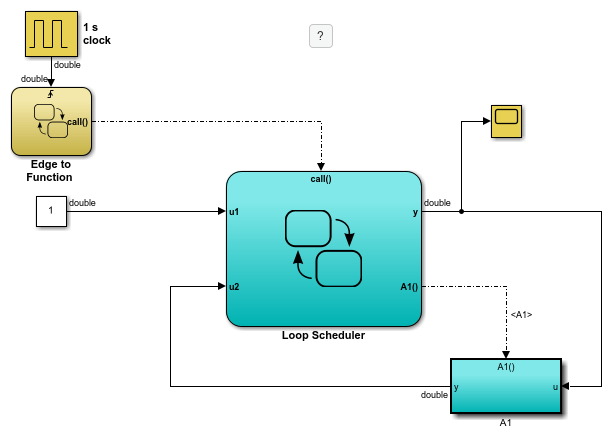
\includegraphics[width=1.0\textwidth]{stateflow.png}
    \end{minipage}%
    \hfill
    \tikz\draw[-{latex}] (0,0) - +(.0818181\textwidth,0) node [midway,above,align=center] {};%
    \hfill
    \begin{minipage}[c]{.2454\textwidth}
      \centering
      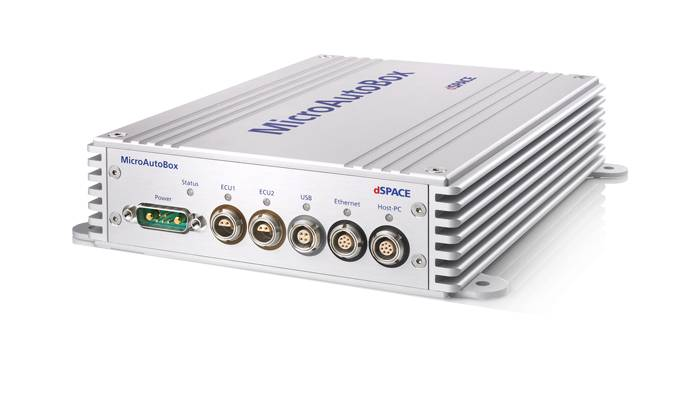
\includegraphics[width=1\textwidth]{microAutoBox.jpeg}
    \end{minipage}
    \hfill
    \tikz\draw[-{latex}] (0,0) - +(.0818181\textwidth,0) node [midway,above,align=center] {};%
    \hfill
    \begin{minipage}[c]{.2454\textwidth}
      \centering
      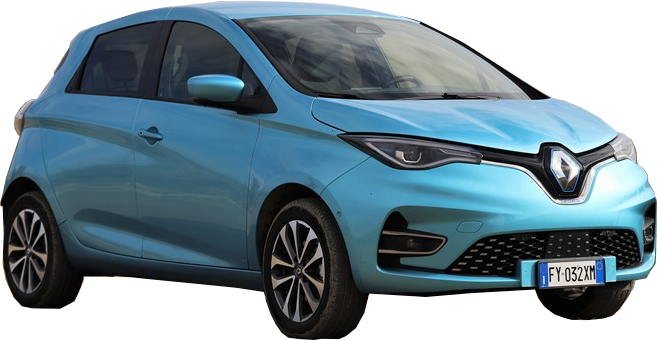
\includegraphics[width=1\textwidth]{zoe.png}
    \end{minipage}
  \end{minipage}
  }
  \vspace{.05cm}
  \only<3->{
    \footnotesize
  \begin{minipage}[c]{.1\linewidth}
    
\includegraphics[width=\textwidth]{logos/poli-ufrj.png}
    
\includegraphics[width=\textwidth]{logos/ufrj.jpeg}%
  \end{minipage}
  \begin{minipage}[c]{.6\linewidth}
    \begin{itemize}
      \item[] Ingénieur (2019)
      \item[] \textit{Identification des SED pour le diagnostic de fautes}
      \item[] Superviseur Marcos Vicente de Brito Moreira
    \end{itemize}
  \end{minipage}
  \begin{minipage}[c]{.25\linewidth}
    \centering
      \begin{minipage}[c]{.4\textwidth}
  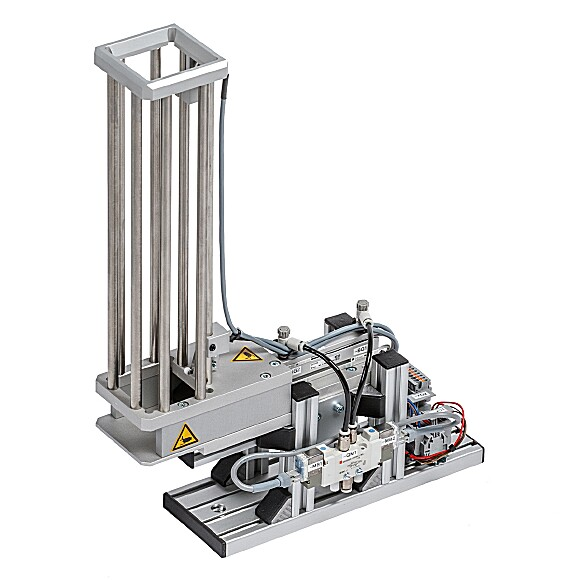
\includegraphics[width=.45\textwidth]{maquete/mag.jpg}
  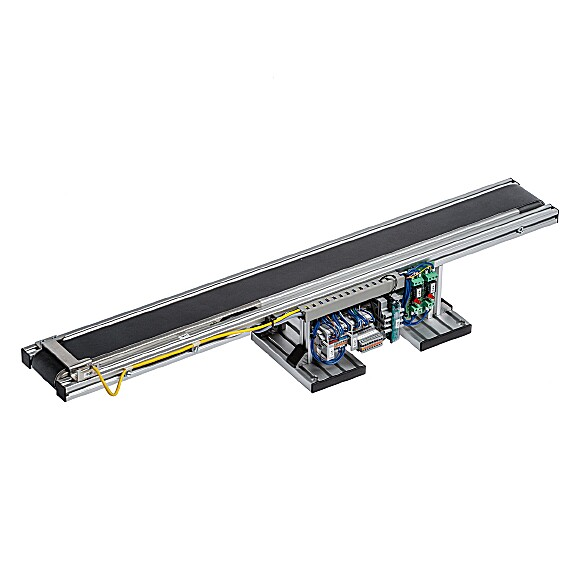
\includegraphics[width=.45\textwidth]{maquete/esteira.jpg}

  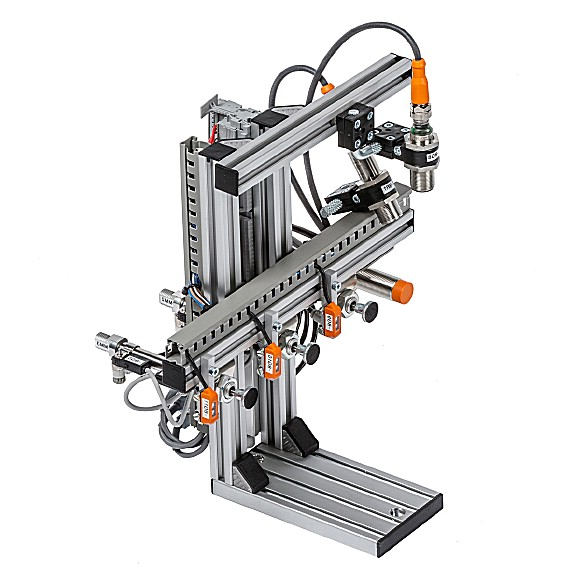
\includegraphics[width=.45\textwidth]{maquete/sensores.jpg}
  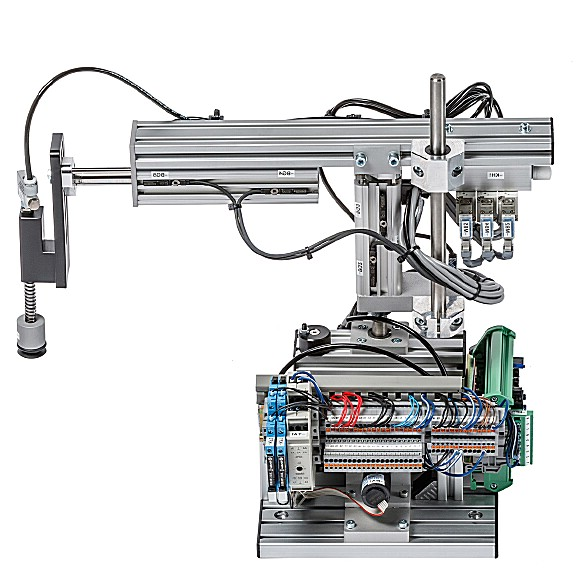
\includegraphics[width=.45\textwidth]{maquete/braco.jpg}

  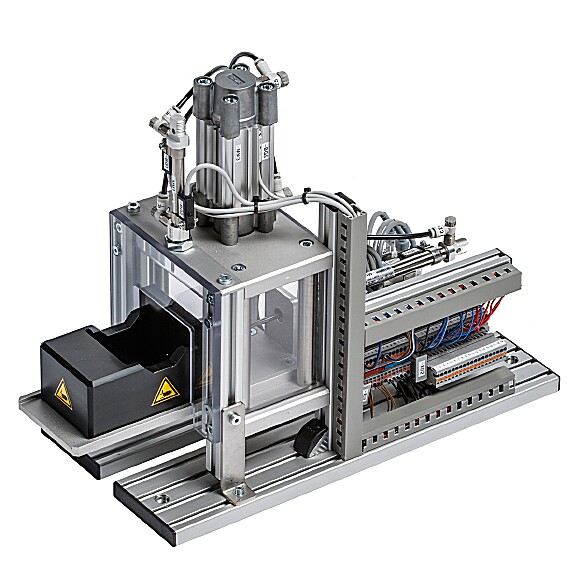
\includegraphics[width=.45\textwidth]{maquete/prensa.jpg}
  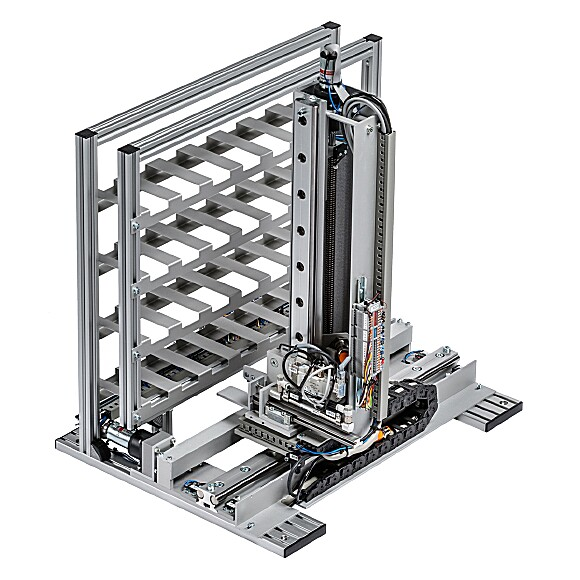
\includegraphics[width=.45\textwidth]{maquete/elevador.jpg}
  \end{minipage}%
  \tikz\draw[-{latex}] (0,0) - +(.1\textwidth,0) node [midway,above,align=center] {I/O\\ +\\ DAOCT};%
  \begin{minipage}[c]{.4\textwidth}
  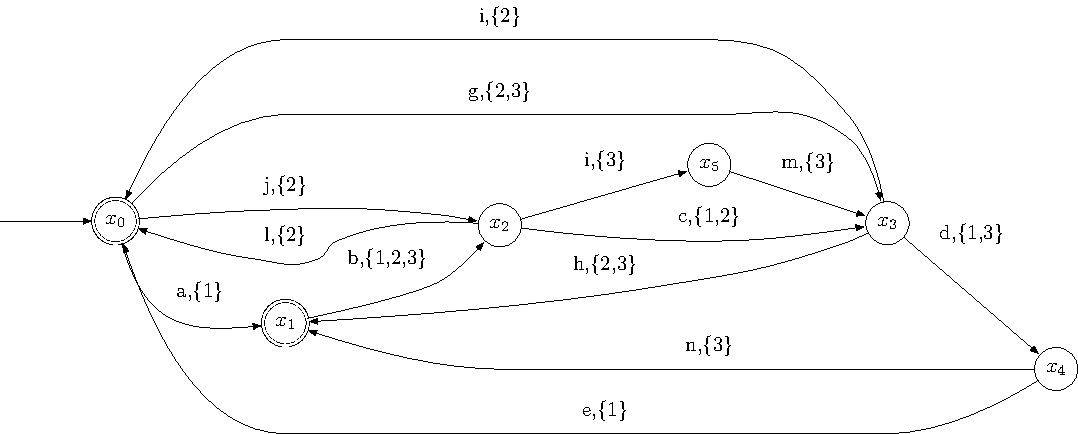
\includegraphics[width=1.5\textwidth]{maquete/example.pdf}
  \end{minipage}
  \end{minipage}
  }

  \vspace{.25cm}
  \only<4->{
  \begin{minipage}[c]{.1\linewidth}
    \centering
    
\includegraphics[width=.8\textwidth]{logos/supelec.jpeg}
    
\includegraphics[width=.8\textwidth]{logos/rennes1.png}
    
\includegraphics[width=.5\textwidth]{logos/IETR_2022.png}%
  \end{minipage}
    \begin{minipage}[c]{.6\linewidth}
    \begin{itemize}
      \item[] Thèse (2022)

      \item[] \textit{Sécurité de dMPC sous False Data Injection}
      \item[] Superviseurs Hervé Guéguen et Romain Bourdais
    \end{itemize}
  \end{minipage}
  \hfill
  \begin{minipage}[c]{.2\linewidth}
    \centering
  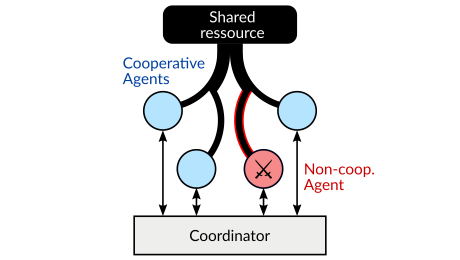
\includegraphics[width=\textwidth]{Non-coop_Agent_1.png}%
  \end{minipage}
  \centering
  }
  \end{overlayarea}
\end{frame}

\begin{frame}{Que fais-je ici?}
  \begin{minipage}[c]{.7\linewidth}
    \begin{itemize}
      \item[] Post-doc mai 2023/mai 2024
      \item[] \textit{Localisation relative garantie dans le scenario anticollision des véhicules autonomes}
      \item[] Plateforme \autOCampus\ (GIS \neOCampus)
    \end{itemize}
  \end{minipage}
  \hfill
  \begin{minipage}[c]{.2\linewidth}
    \centering
    
\includegraphics[width=3cm]{logos/laas-logo.png}%
    \\~\\%
    
\includegraphics[width=3cm]{ups-logo}%
  \end{minipage}
\end{frame}

\begin{frame}{À propos de la plateforme \autOCampus}
  \pause
  «Plateforme d'expérimentation sur la mobilité du futur»\pause

  Le campus de Rangueil : une « smart city »  \pause

  https://www.irit.fr/autocampus/ \pause

  \begin{minipage}[c]{.45\linewidth}
    \begin{itemize}
      \item Simulateur SimFlex
      \item Navette et droïdes autonomes
      \item Véhicule autonome open source
      \item Lampadaires intelligents
      \item 5G privée (V2X)
      \item Datalake
      \item Centre de supervision
    \end{itemize}

  \end{minipage}
  \hfill
  \begin{minipage}[c]{.3\linewidth}
    \centering
    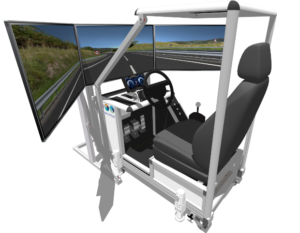
\includegraphics[width=.35\textwidth]{simflex}%
    \hfill
    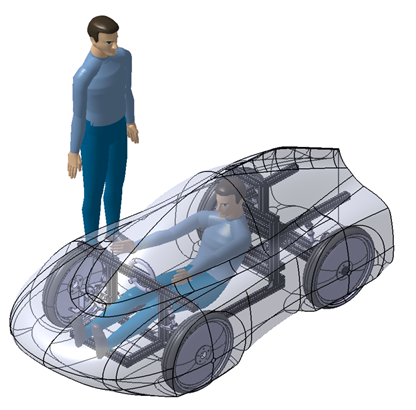
\includegraphics[width=.35\textwidth]{vacop}%

    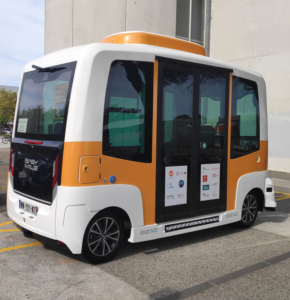
\includegraphics[width=.35\textwidth]{navette}%
    \hfill
    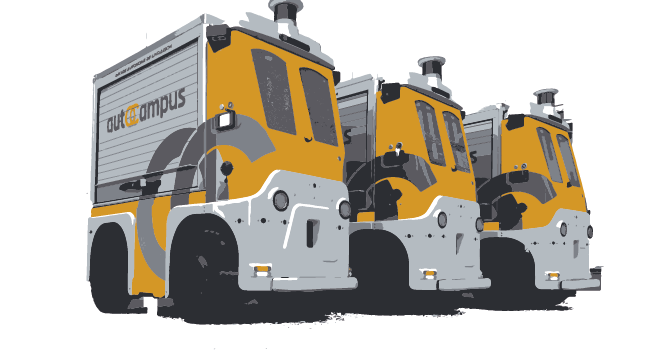
\includegraphics[width=.45\textwidth]{twinswheel}%

    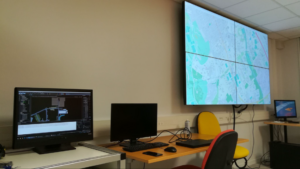
\includegraphics[width=.8\textwidth]{centre_supervision}%
  \end{minipage}

    \pause
    Nous serons un des premiers utilisateurs de la plateforme

\end{frame}

\begin{frame}{Problème: Navigation sans collision}
  \begin{minipage}[c]{.45\linewidth}
    \structure{\underline{On a plusieurs scénarios de navigation}}

    \begin{itemize}
      \item Carrefours
      \item Dépassements
      \item Circulation en peloton
      \item ...
    \end{itemize}

    \onslide<+(1)->{Localisation absolue n'est pas nécessaire}

    \onslide<+(1)->{Distances relatives} \onslide<+(1)->{$\to$ \alert{zones interdites}}

    \onslide<+->{\[{\alert{\set{D}_{i}}\ni\vec{d}_{i,j}=\vec{p}_{j}-\vec{p}_{i}}\]}

    \onslide<+(1)->{Utiliser les $\set{D}_{i}$ pour des algorithmes de navigation}
  \end{minipage}
  \hfill
  \begin{minipage}[c]{.45\linewidth}
    \begin{tikzpicture}
      \node[alt=<{2-}>{opacity=0.2}] (0,0) {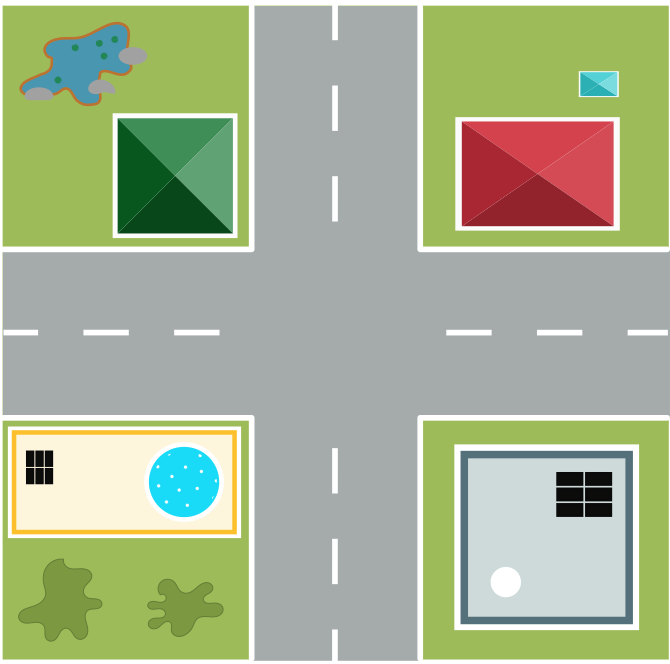
\includegraphics[width=.7\textwidth]{crossroad.png}};

      \node (car_red) at (0.25,-1) {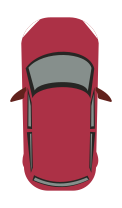
\includegraphics[height=.75cm]{car_red}};

      \node[above right=.9cm of car_red] (car_purple_position) {};
      \onslide<.->{
      \path[draw,use Hobby shortcut,closed=true,violet!50!white,fill=violet!50!white,opacity=0.75]
($(car_purple_position)+(.5,0)$) .. ++(-.3,.3) .. ++(-.1,.05) .. ++(-0.6,-0.1) ..++(-0.1,-0.4) ..++(0.2,-0.1);
}
      \node[] (car_purple) at (car_purple_position) {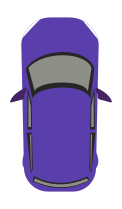
\includegraphics[height=.75cm,angle=90]{car_purple}};

      \node[above left=-.2cm and 1cm of car_purple] (car_brown_position) {};
      \onslide<.->{
      \path[draw,use Hobby shortcut,closed=true,olive!50!white,fill=olive!50!white,opacity=0.75]
($(car_brown_position)+(.2,-.5)$) .. ++(.1,.5) .. ++(-.04,.4) .. ++(-0.5,-0.3);}
      \node (car_brown) at (car_brown_position) {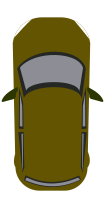
\includegraphics[height=.75cm]{car_brown}};

    \end{tikzpicture}

  \end{minipage}


\end{frame}

\begin{frame}{Stratégie usuelle: Estimation Bayésienne (Kalman)}
  \begin{itemize}
    \item Modèles dynamiques pour prédire état
    \item Capteurs embarqués pour corriger prédictions du modèle
  \end{itemize}
  ~\\[.2cm]

  \only<2->{Examples de «capteurs» embarqué dans une voiture}

  \only<3->{
    \begin{minipage}[t]{.3\linewidth}
    \begin{itemize}
      \item \alert<4>{D-GNSS} \onslide<4->{(code phase)}
      \item Sonar
    \end{itemize}
  \end{minipage}
  \begin{minipage}[t]{.4\linewidth}
    \begin{itemize}
      \item \alert<4>{Ultra-Wideband} \onslide<4->{(range)}
      \item Lidar
    \end{itemize}
  \end{minipage}
  \begin{minipage}[t]{.2\linewidth}
    \begin{itemize}
      \item Odométrie
      \item ...
    \end{itemize}
  \end{minipage}
  }
    ~\\[.1cm]

    \begin{overlayarea}{\textwidth}{\textheight}
      \onslide<4->{\alert<4>{\[\nabla^{r}\rho_{p,i,j}=\norm{\vec{p}_{i}-\vec{p}_{j}}%
          -\norm{\vec{p}_{i}+\text{\structure<5>{$\vec{d}_{i,j}$}}-\vec{p}_{s}}%
          -\norm{\vec{p}_{i}-\vec{p}_{r}}%
          +\norm{\vec{p}_{i}+\text{\structure<5>{$\vec{d}_{i,j}$}}-\vec{p}_{r}}%
          +\nabla^{r}\epsilon_{p,i,j}\]}}
    \vspace{-1cm}

    \onslide<4->{\alert<4>{\[r_{i,j}=\norm{\text{\structure<5>{$\vec{d}_{i,j}$}}}+w_{r}\]}}

    \vspace{-.5cm}
    \onslide<6->{$\norm{\cdot}$ $\to$ Non-linéaire $\to$ Extensions non-linéaires du Filtre de Kalman (EKF, UKF, etc)}

    \end{overlayarea}
\end{frame}

\begin{frame}{Estimation Bayésienne: EKF, UKF}

  \begin{minipage}{.45\linewidth}
  \begin{block}{Hypothèses}
    \begin{enumerate}
      \item Bruit d'évolution\tikzmark{a}
      \item Bruit de mesure
    \end{enumerate}
    \onslide<+(1)->{\begin{tikzpicture}[overlay, remember picture,decoration={brace,amplitude=2pt}]
      \draw[decorate,thick] (a.north east) --+ (0,-1) node[midway, right,text=black,align=center] {Gaussiens\\ et\\ connus};
    \end{tikzpicture}%
    }

  \end{block}
  \end{minipage}
  \hfill
  \visible<+(1)->{\tikz\draw[-{latex},line width=1pt] (0,0) -++(1,0);}
  \hfill
  \begin{minipage}{.45\linewidth}
    \visible<+->{
    \begin{block}{Résultat = Erreur Gaussien}
      Intervalles de confiance = ellipsoïdes
      \begin{itemize}
        \item<+-> $3\sigma=99.73\%$
        \item<+-> $4\sigma=99.993\%$
      \end{itemize}
    \end{block}}
  \end{minipage}

  \centering
  \begin{tikzpicture}[scale=0.5]
    \node at (0,0) (car_red_position) {};
    \node (car_red) at (car_red_position) {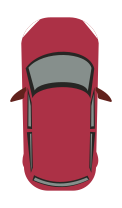
\includegraphics[height=1cm]{car_red}};

    \node[above right=.6cm of car_red] (car_purple_position) {};
    \onslide<5->{\draw[rotate=20,violet!50!white,fill=violet!50!white,opacity=0.75] (car_purple_position) ellipse (2cm and 1cm);}
    \onslide<4->{\draw[rotate=20,violet!100!white,fill=violet!100!white,opacity=0.75] (car_purple_position) ellipse (1cm and .5cm);}
    \node (car_purple) at (car_purple_position) {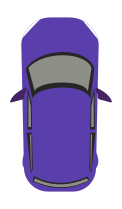
\includegraphics[height=1cm,angle=90]{car_purple}};

    \node[above right=.75cm of car_purple] (car_brown_position) {};
    \onslide<5->{\draw[rotate=0,olive!50!white,fill=olive!50!white,opacity=0.5] (car_brown_position) ellipse (1.2cm and 1cm);}
    \onslide<4->{\draw[rotate=0,olive!100!white,fill=olive!100!black,opacity=0.5] (car_brown_position) ellipse (0.6cm and .5cm);}
    \node (car_brown) at (car_brown_position) {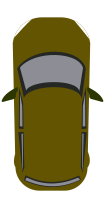
\includegraphics[height=1cm]{car_brown}};

    \node (car_red) at (car_red_position) {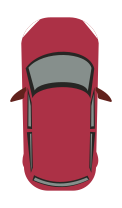
\includegraphics[height=1cm]{car_red}};
    \draw[-{latex},line width=1pt] (-.5,0) -- (5,0);
    \draw[-{latex},line width=1pt] (0,-0.5) -- (0,5);

  \end{tikzpicture}

\end{frame}

\begin{frame}{Estimation Bayésienne: EKF, UKF}{Problème dans les hypothèses}
  \begin{minipage}{.45\linewidth}
    \begin{block}{Hypothèses}
      \begin{enumerate}
        \item Bruit d'évolution\tikzmark{a}
        \item Bruit de mesure
      \end{enumerate}
      \begin{tikzpicture}[overlay, remember picture,decoration={brace,amplitude=2pt}]
        \draw[decorate,thick] (a.north east) --+ (0,-1) node[midway, right,text=black,align=center] {Gaussiens\\ et\\ connus};
      \end{tikzpicture}%
    \end{block}
  \end{minipage}
  \hfill
  \visible<+(1)->{\tikz\draw[-{latex},line width=1pt] (0,0) -++(1,0);}
  \hfill
  \begin{minipage}{.45\linewidth}
    \begin{tikzpicture}
      \onslide<2->{
        \node {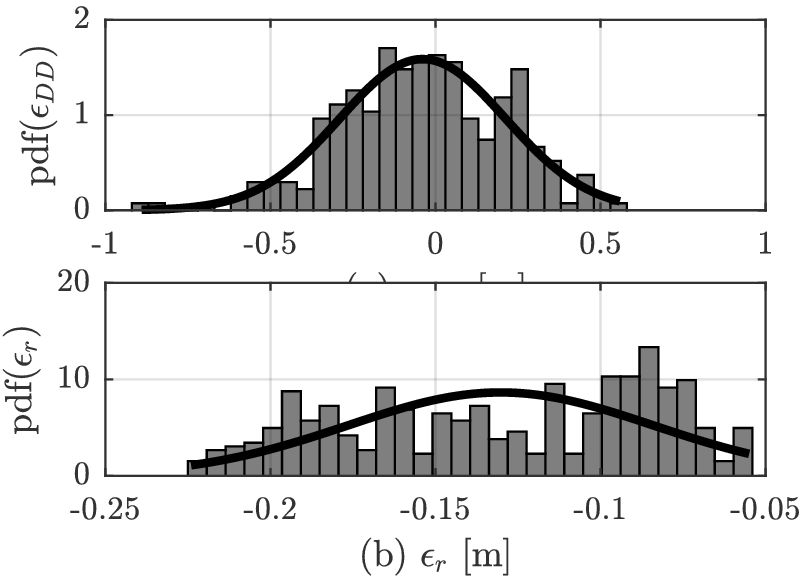
\includegraphics[width=0.7\textwidth]{normal_sensor}};
      }
      \onslide<3->{
        \draw[-{latex},line width=1pt,neocampus_yellow] (0,.5) -- (3,1) node[red,right] {pas vrai!};
        \draw[-{latex},line width=1pt,neocampus_yellow] (0,-.5) -- (3,1);
      }
    \end{tikzpicture}
  \end{minipage}

  \onslide<4->{
  \begin{minipage}[c]{.45\textwidth}
    \scalebox{0.8}{
    \begin{tikzpicture}[spy using outlines={circle, magnification=4, size=2cm, connect spies}]
      \node {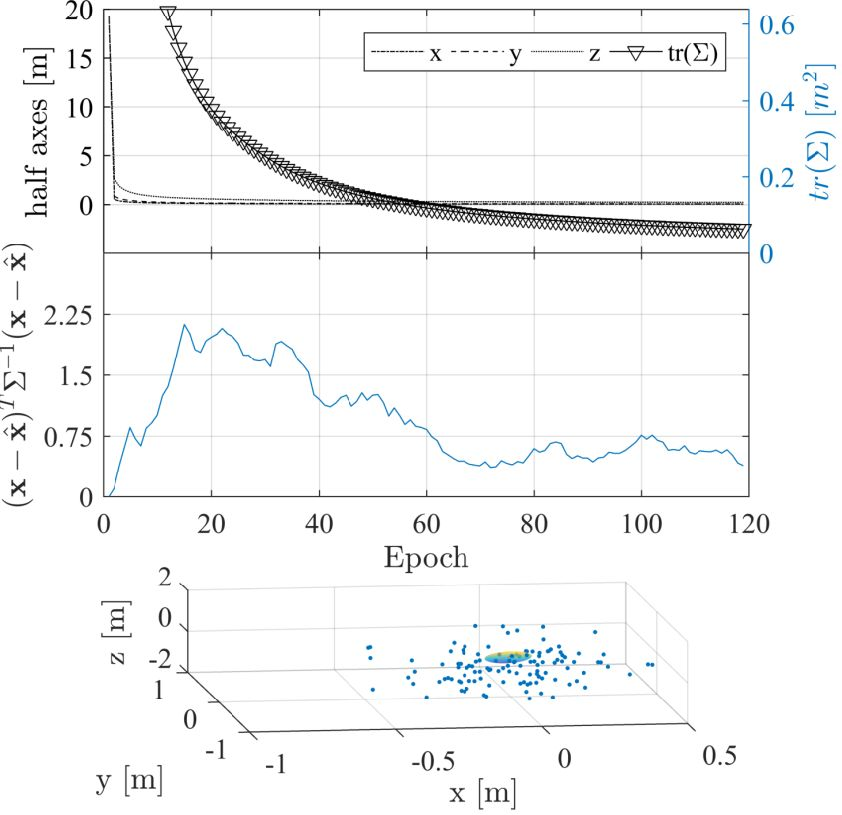
\includegraphics[width=0.7\textwidth]{real_position}};
      \onslide<6->{
        \draw[-{latex},line width=1pt,neocampus_yellow] (-1.,.5) -- (3,1) node[red,right,align=center] {points \\dehors\\ ellipsoïde};
        \draw[-{latex},line width=1pt,neocampus_yellow] (0,-1.2) -- (3,1);

      }
      \only<5->{\spy on (0.45,-1.3) in node at (3,-.7);}
    \end{tikzpicture}
    }
  \end{minipage}}
\end{frame}

\begin{frame}{Alternative: Méthodes ensemblistes}

  \onslide<2->{
  \begin{block}{Hypothèse principale}
    \begin{itemize}
      \item On ne connaît pas la distribution des erreurs, mais ses \tikzmarktext{b}{bornes}
    \end{itemize}
  \end{block}
  }
  \onslide<4->{
  \begin{itemize}
    \item Garantie que les valeurs appartiennent à l'intervalle
    \item Intervalle + dynamiques génèrent un ensemble garanti \onslide<5->{(mais de \tikzmarktext{a}{forme inconnue} \frownie)}
  \end{itemize}
  }
  \onslide<1->{
  \begin{minipage}[c]{1\textwidth}
    \centering
    \scalebox{0.75}{
      \begin{tikzpicture}
        \node {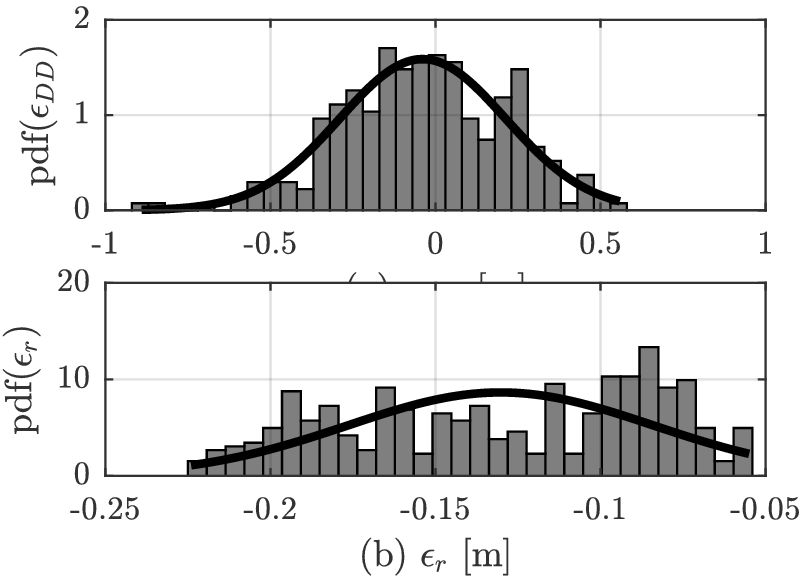
\includegraphics[width=0.45\textwidth]{normal_sensor}};
        \draw<2->[fill=neocampus_bright_yellow,opacity=0.5,draw=none] (-2.15,0.6) rectangle ++(4,1.5);
        \draw<2->[fill=neocampus_bright_yellow,opacity=0.5,draw=none] (-1.7,-1.45) rectangle ++(4.5,1.5);
      \end{tikzpicture}
    }
    }

  \end{minipage}
  \begin{minipage}{\textwidth}
    \onslide<3->{\tikz[overlay,remember picture]\draw[-{latex}] (b) -- +(30:1.) node[above] {Datasheet + Erreur Modélisation};}
  \end{minipage}

  \begin{minipage}{\textwidth}
    \onslide<6->{\tikz[overlay,remember picture]\draw[-{latex}] (a) -- +(30:1.) node[above ] {On peut l'approximer \smiley};}
  \end{minipage}

\end{frame}

\begin{frame}{Approximation par ensembles connus}
  \centering
  \begin{overlayarea}{\textwidth}{.25\paperheight}
    \begin{itemize}
      \item<+(1)-> Compromis entre complexité de calcul et conservatisme
            \begin{itemize}
              \item<+(1)-> Rapide mais conservative: {\color<3>{green!50!white}{intervalles}}, {\color<4>{blue!50!white}{ellipsoïdes}}, {\color<5>{olive!50!white}{zonotopes}}
              \item<+(3)-> Lent mais serré (normalement hors-ligne): \alert<6>{sous-pavage (SIVIA)}, {\color<7>{neocampus_yellow}{polytopes}}
            \end{itemize}
      \item<+(4)-> Zonotope Contraint\only<.(4)->{\footnote{\cite{ScottEtAl2016} (\citeyear{ScottEtAl2016})} }(une autre representation de polytopes)
    \end{itemize}
  \end{overlayarea}

  \vfill
  \begin{overlayarea}{\textwidth}{.3\paperheight}
    \begin{minipage}[c]{.45\linewidth}
      \scalebox{3}{
        \begin{tikzpicture}
          % \draw [help lines] (-1,-1) grid [step=.1cm] (1,1);
          \node[] (car_purple_position) {};

          % interval
          \onslide<3->{
            \draw[green!50!white,fill=green!50!white,alt=<4->{opacity=0.2}] (-0.65,-0.33) rectangle ++(1.15,.73);
          }

          % ellipse
          \onslide<4->{
            \draw[rotate=20,blue!50!white,fill=blue!50!white,alt=<5->{opacity=0.2}] ($(car_purple_position)+(-0.075,0)$) ellipse (.7cm and .44cm);
          }

          % zonotope
          \onslide<5->{
            \def\s{0.42}
            \def\a{0.88}
            \draw[olive!50!white,fill=olive!50!white,xshift=-0.71cm,yshift=0.04cm,alt=<6->{opacity=0.2}] (0,0) -- ++(60:\s) -- ++(0:\a) --++(-60:\s) -- ++(240:\s) --++(180:\a) -- ++(120:\s);
          }

          % constrained zonotope/ polytope
          \onslide<7->{
            \draw[neocampus_yellow,fill=neocampus_yellow] (-0.65,-0.1) -- ++(90:0.2) -- ++(45:0.42) --++(0:0.4) -- ++(-30:0.53) -- ++(-90:0.32) -- ++(210:0.28) --++(180:0.45) --++(160:0.49) -- cycle;
          }

          \path[draw,use Hobby shortcut,closed=true,violet!50!white,fill=violet!50!white]
          ($(car_purple_position)+(.5,0)$) .. ++(-.3,.3) .. ++(-.1,.05) .. ++(-0.6,-0.1) ..++(-0.1,-0.4) ..++(0.2,-0.1);
          \node[] (car_purple) at (car_purple_position) {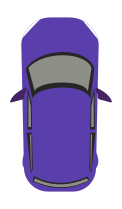
\includegraphics[height=1cm,angle=90]{car_purple}};

        \end{tikzpicture}
      }
    \end{minipage}
    \hfill
    \begin{minipage}[c]{.45\linewidth}
      \visible<6->{
        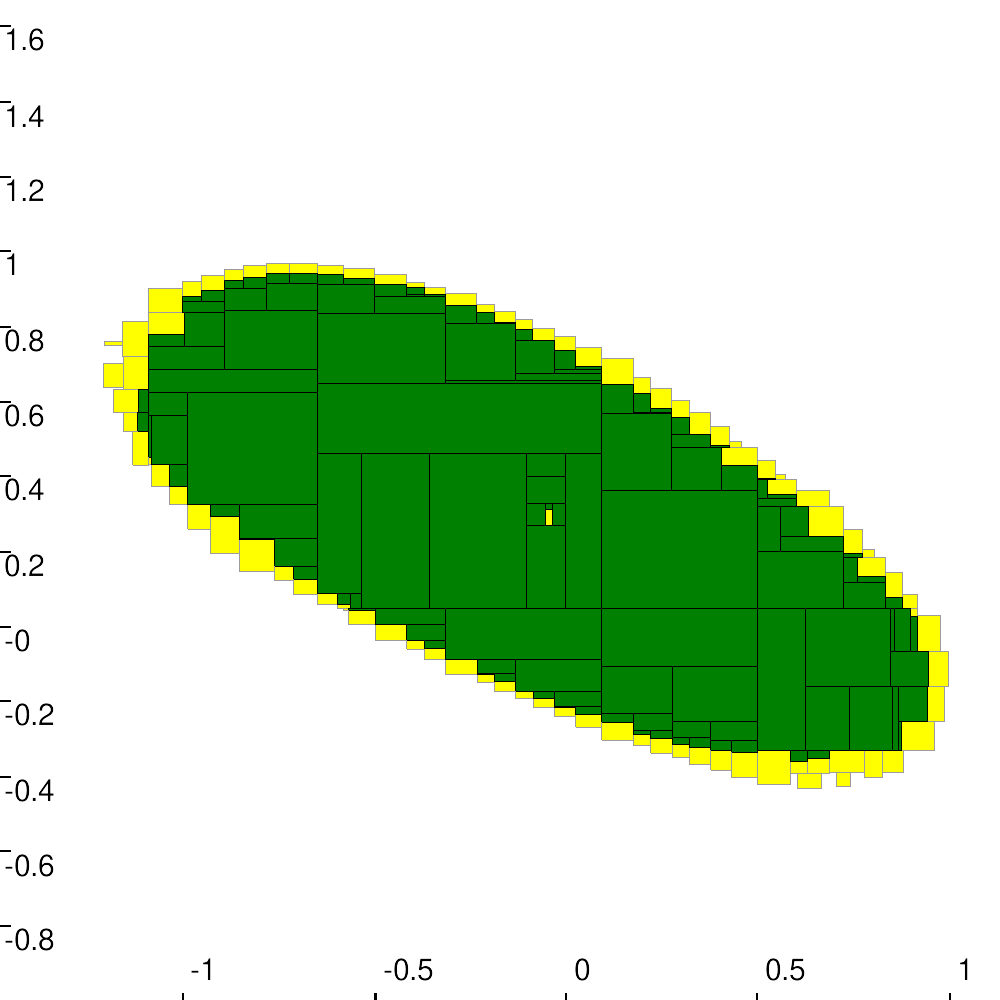
\includegraphics[clip,trim={2 1.5 0 0},width=.6\textwidth]{sivia}
      }
    \end{minipage}
  \end{overlayarea}
\end{frame}

\begin{frame}{Zonotope contraint: }
  \centering
  \begin{itemize}
    \item Propriétés similaires au polytopes (Clos pour l'intersection et somme de Minkowski)
          \begin{itemize}[<+(1)->]
            \item[+] Répresentation facilite exécution des opérations
            \item[+] Asymétrie $\to$ plus de liberté
            \item[+] Facilement appliquable pour des systèmes linéaires
            \item[-] Chaque opération augmente la complexité (réduction possible au détriment du volume)
          \end{itemize}
  \end{itemize}

  \vspace{.25cm}
  \begin{minipage}[c]{.45\linewidth}
    \centering
    \scalebox{3}{
      \begin{tikzpicture}
        % \draw [help lines] (-1,-1) grid [step=.1cm] (1,1);
        \node[] (car_purple_position) {};

        % constrained zonotope
        \draw[neocampus_yellow,fill=neocampus_yellow] (-0.65,-0.1) -- ++(90:0.2) -- ++(45:0.42) --++(0:0.4) -- ++(-30:0.53) -- ++(-90:0.32) -- ++(210:0.28) --++(180:0.45) --++(160:0.49) -- cycle;

        \path[draw,use Hobby shortcut,closed=true,violet!50!white]
        % \path[draw,use Hobby shortcut,closed=true,violet!50!white,fill=violet!50!white,opacity=0.5]
        ($(car_purple_position)+(.5,0)$) .. ++(-.3,.3) .. ++(-.1,.05) .. ++(-0.6,-0.1) ..++(-0.1,-0.4) ..++(0.2,-0.1);
        \node[] (car_purple) at (car_purple_position) {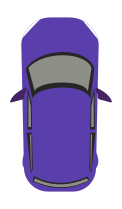
\includegraphics[height=1cm,angle=90]{car_purple}};

      \end{tikzpicture}
    }
    \[\set{C}_{\set{Z}}=\setbuild{G\vec{\xi}+\vec{c}}{\norm{\vec{\xi}}_{\infty}\leq 1,A\vec{\xi}=\vec{b}}\]
  \end{minipage}
\end{frame}

\begin{frame}{Filtre d'estimation avec zonotopes contraints (CZESMF) \hyperlink{czesmf_algo}{\beamergotobutton{plus}}}
\hypertarget{czesmf_presentation}{}
  \begin{minipage}[c]{.6\linewidth}
    \begin{itemize}
      \item Extension pour des systèmes non-linéaires
      \item Extension pour temps d'observation uncertains
      \item Testé (en simulation) avec D-GNSS et UWB p2p
      \item Exécution proche du temps réel (Matlab)
    \end{itemize}
  \end{minipage}
  \begin{minipage}[c]{.3\linewidth}
    \centering
  \scalebox{0.3}{
    \def\svgwidth{10cm}
    \import{../img/}{timing.pdf_tex}
    %	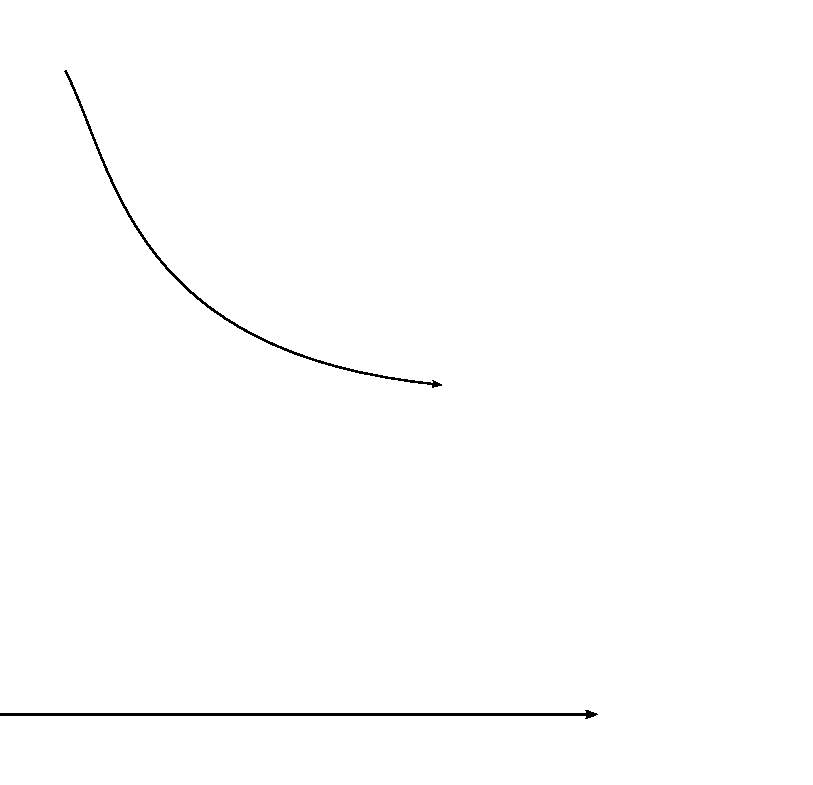
\includegraphics[width=.99\linewidth]{timing.pdf}
  }
  \end{minipage}

  \visible<2->{
    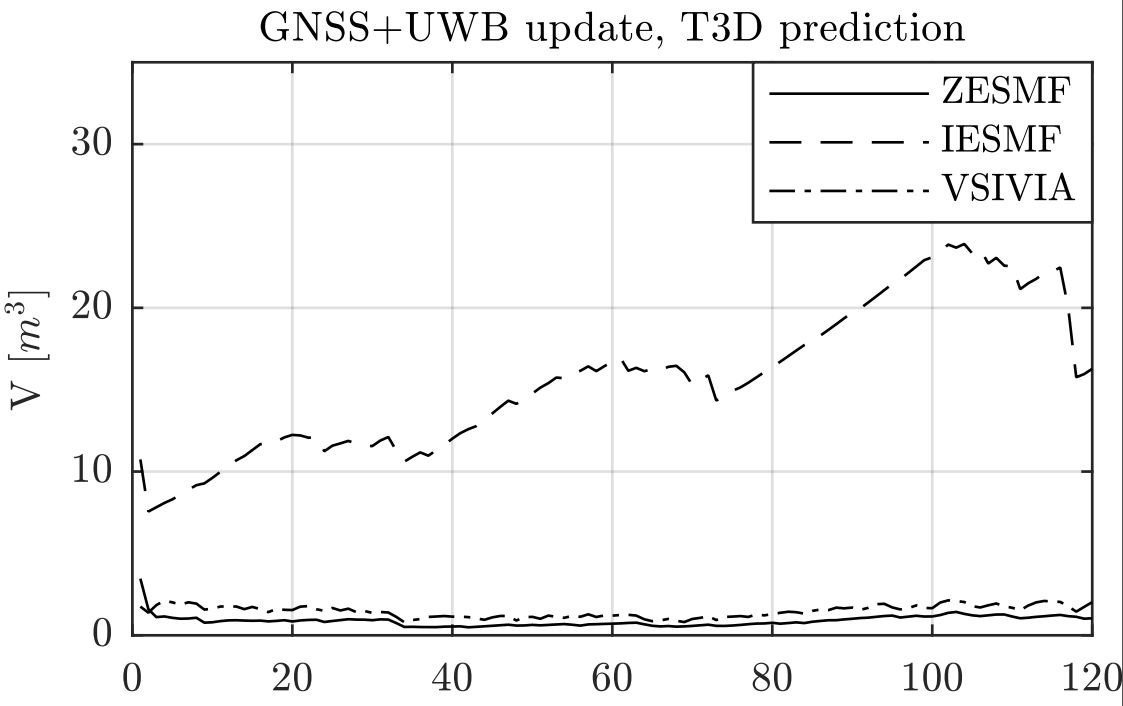
\includegraphics[clip,trim=0 0 0.075cm 0,width=.4\textwidth]{volumes_comparison}%
    \hfill
    \resizebox{.4\textwidth}{!}{

      \begin{tikzpicture}[spy using outlines={circle, magnification=4, size=2cm, connect spies}]
        % \draw [help lines] (-3,-1) grid [step=.5cm] (1,2);
        \node[] {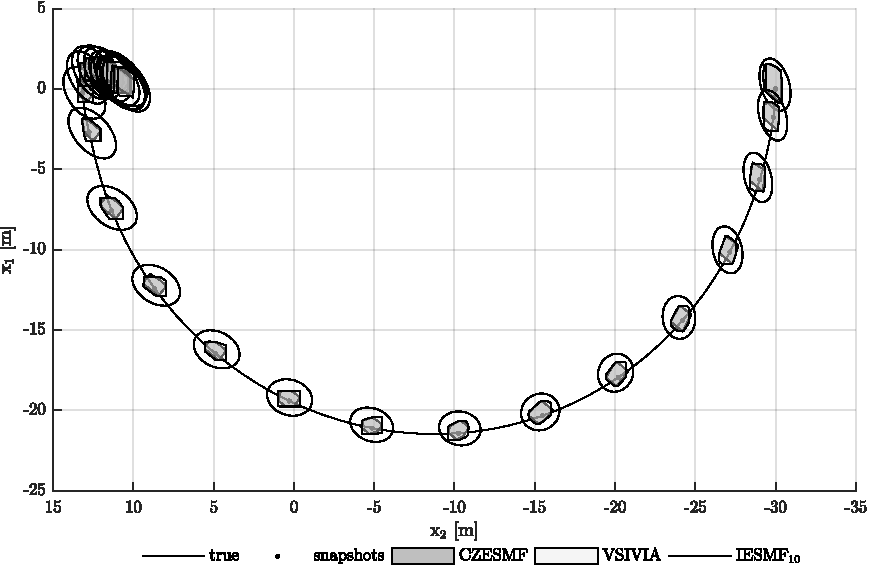
\includegraphics[width=5.5cm]{comparison_czesmf_vsivia_IESMF.pdf}};
        \node (car_red) at (0.1,1.2) {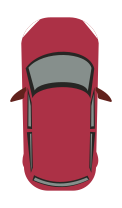
\includegraphics[height=.75cm]{car_red}};
        \node[rotate=20] (car_purple) at (-2,0.5) {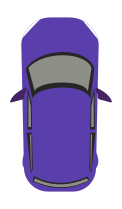
\includegraphics[height=.75cm]{car_purple}};
        \only<3->{\spy on (0.15,-.9) in node at (1.6,.7);}
      \end{tikzpicture}

    }
  }
\end{frame}

\begin{frame}{Mission}
  \begin{minipage}[c]{.6\textwidth}
    \begin{enumerate}
      \item Validation de l'algorithme dans une cible
            \begin{itemize}
              \item Quanser QBot 3 (Raspberry Pi 4 Model B)
                    \begin{itemize}
                      \item IMU
                      \item Odométrie
                      \item Caméra
                      \item ...
                    \end{itemize}
              \item Tâches
                    \begin{itemize}
                      \item Configuration Robot
                      \item Intégration code C++ et tests
                      \item Adaptation (dynamique et capteurs)
                      \item Environnement Simulation (ROS)
                      \item Création démonstrateur
                    \end{itemize}
            \end{itemize}
    \end{enumerate}
  \end{minipage}
  \hfill
  \begin{minipage}[c]{.3\textwidth}
    \resizebox{\textwidth}{!}{
      \begin{tikzpicture}
        \clip[] (0,0) circle (1.5cm);
        \node {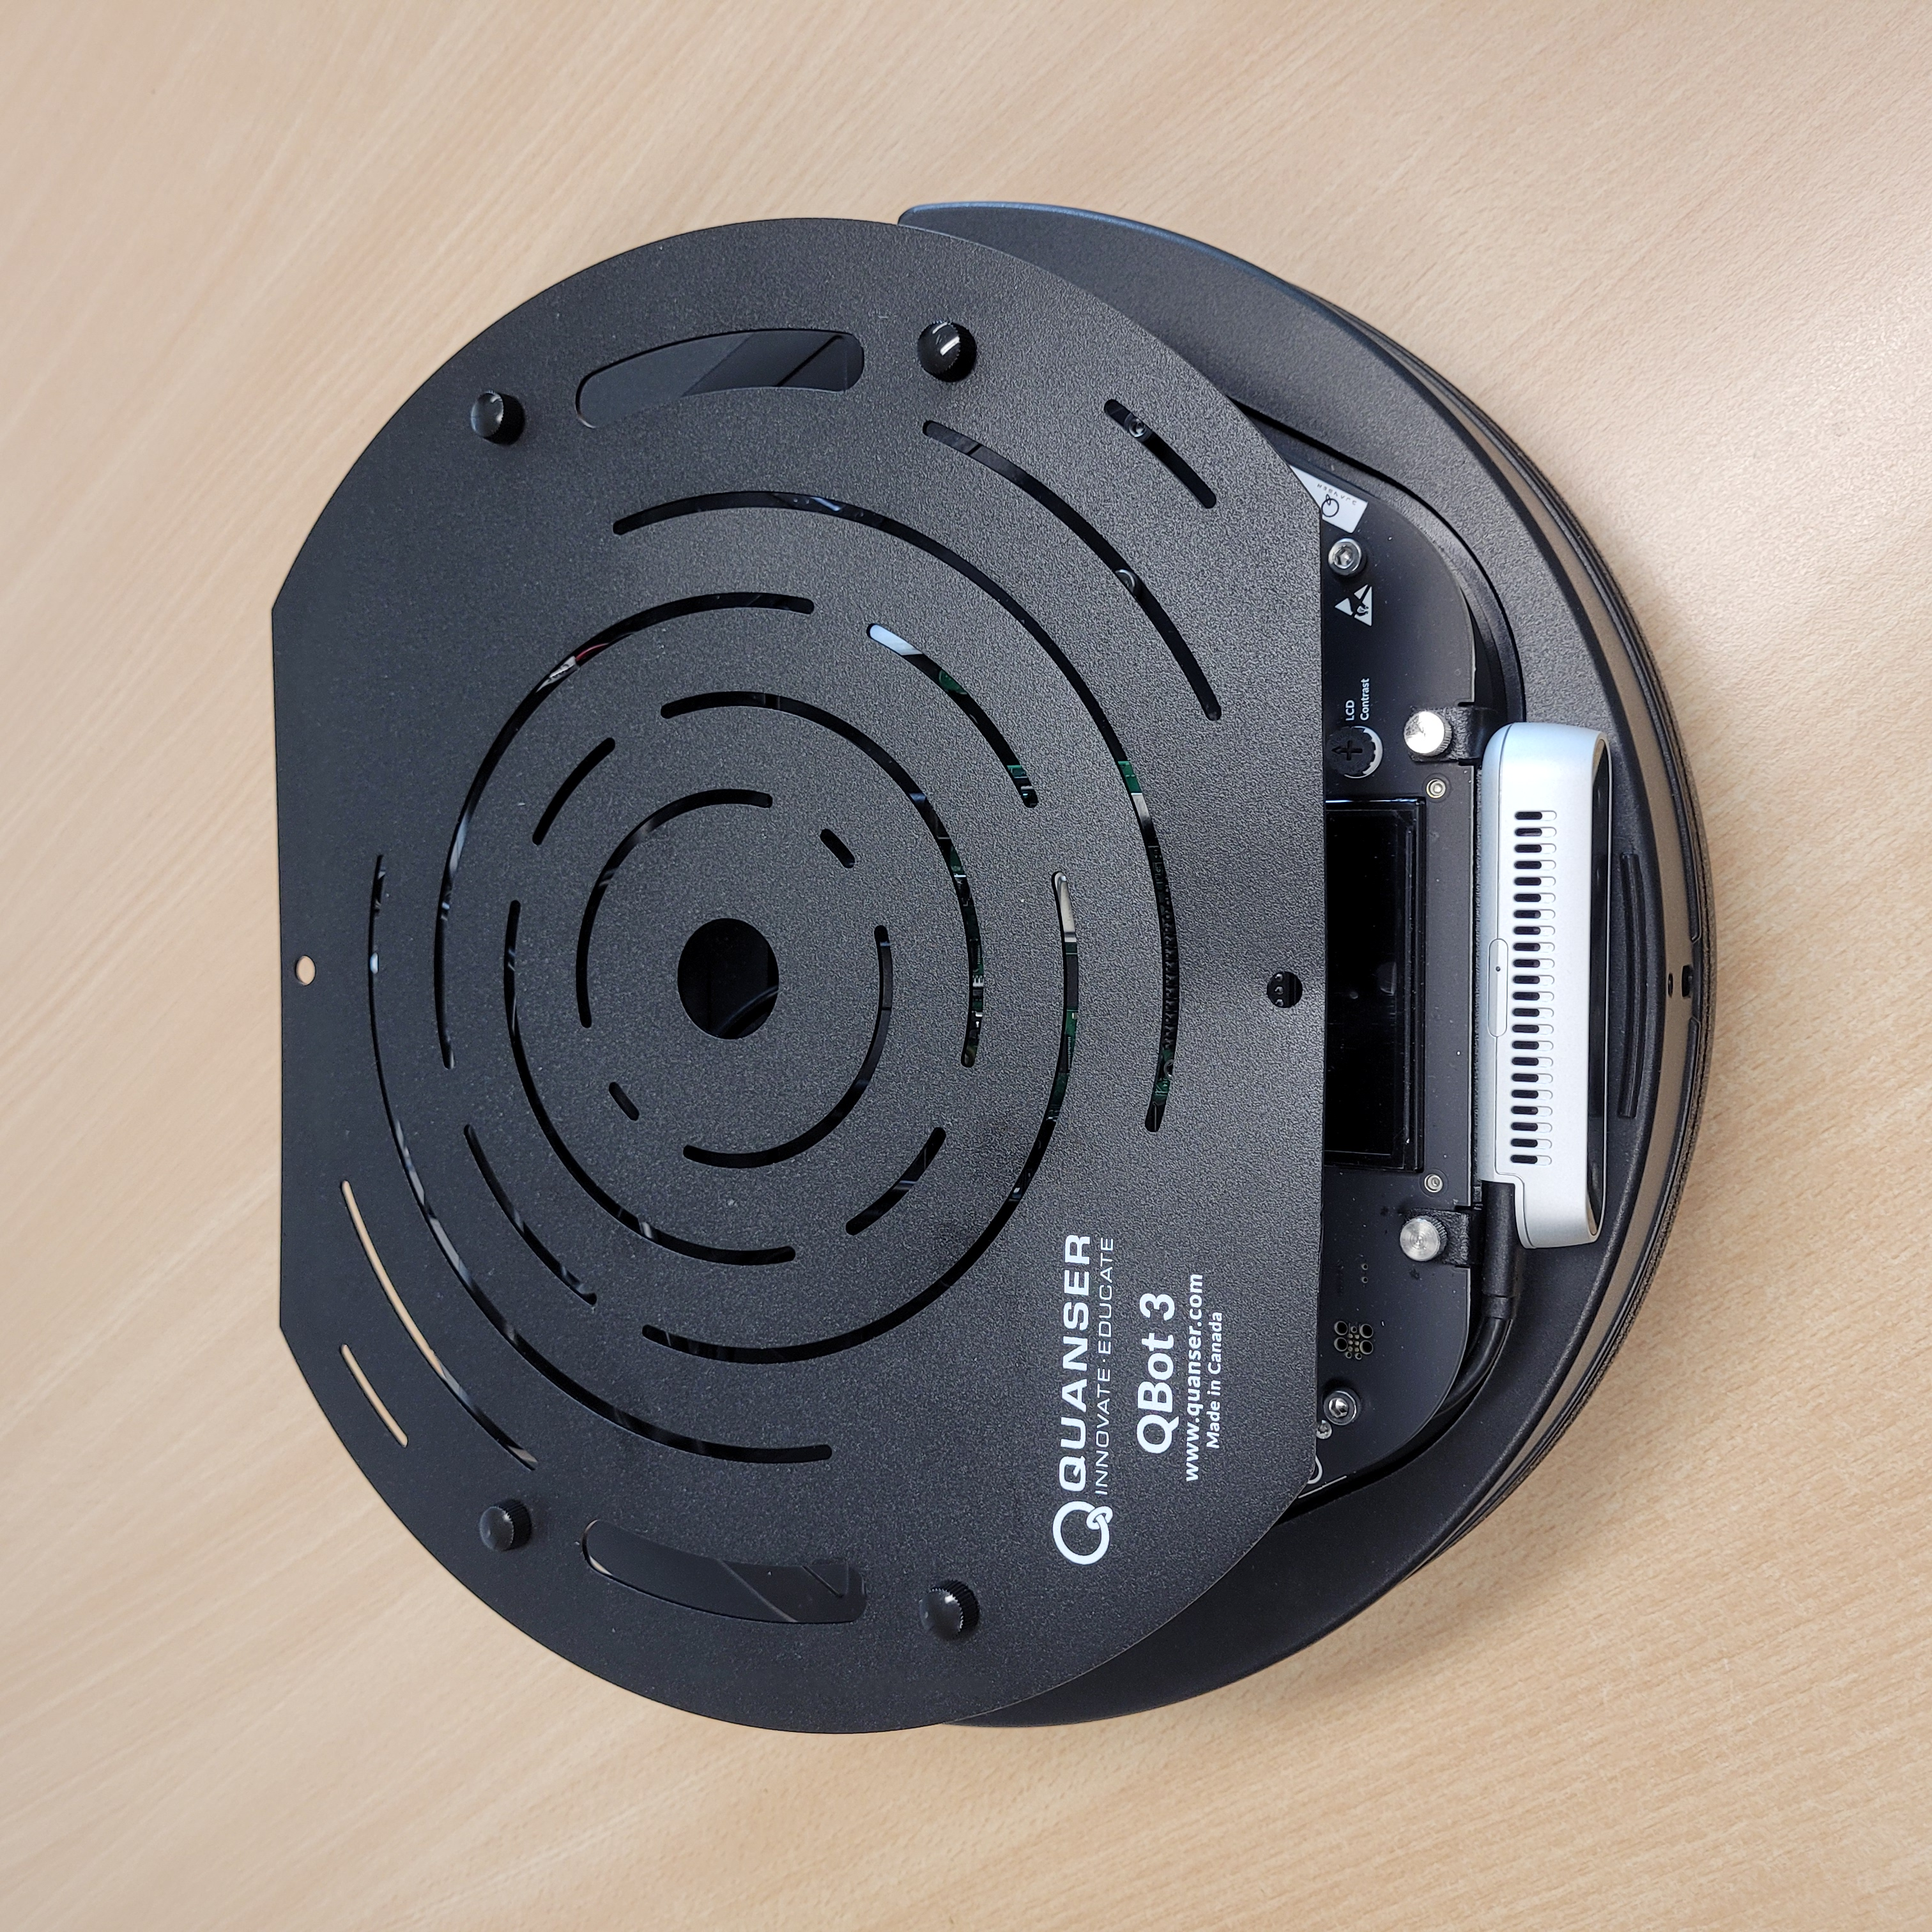
\includegraphics[angle=-90,width=3cm]{qbot3}};
      \end{tikzpicture}
    }
  \end{minipage}
\end{frame}

\begin{frame}{Mission - Perspective}
  \begin{minipage}[c]{.6\textwidth}
    \begin{enumerate}
            \setcounter{enumi}{1}
      \item Application: Droïdes TwinswHeel
            \begin{itemize}
              \item Données GNSS réeles du campus
              \item Adaptation (dynamique et capteurs)
              \item Tests en simulation (ROS)
              \item Intégration sur les droïdes
            \end{itemize}
    \end{enumerate}
  \end{minipage}
  \hfill
  \begin{minipage}[c]{.35\textwidth}
    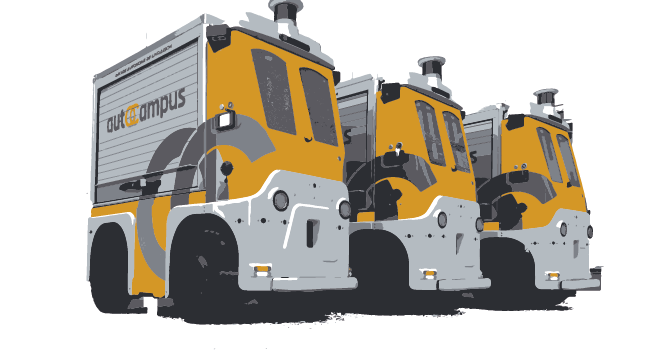
\includegraphics[width=1\textwidth]{twinswheel}%
  \end{minipage}
\end{frame}

\begin{frame}[plain]
  \centering
  \vskip1.5cm
  Merci! Questions?
  \vskip1.5cm
  
\includegraphics[width=0.8\textwidth]{autocampus-logo.png}
  \vskip.5cm
  \begin{center}
    \insertauthor
  \end{center}
  \tikz[remember picture,overlay]\node[anchor=south west,align=center] at ([yshift=0.2cm,xshift=0.25cm]current page.south west){
    \includegraphics[width=2cm]{laas-logo}%
  };
  \tikz[remember picture,overlay]\node[anchor=south east,align=center] at ([yshift=0.2cm,xshift=-0.25cm]current page.south east){
    \includegraphics[width=3cm]{ups-logo}%
  };

\end{frame}

\appendix

\begin{frame}{CZESMF - L'algorithme \hyperlink{czesmf_presentation}{\beamerreturnbutton{}}}
\hypertarget{czesmf_algo}{}
\centering
Équations d'état et d'observation (Horodatage incluse)
\begin{equation*}
  \begin{matrix}
  \vec{x}_{t_{k+1}}&=&f(\vec{x}_{t_{k}},\vec{u}_{t_{k}},t_{k+1},t_{k})&+&\vec{q}_{t_{k}}\\
    \vec{y}_{t_{y,k+1}} &=& h(\vec{x}_{t_{y,k+1}},\vec{u}_{t_{y,k+1}},t_{y,k+1})&+&\vec{w}_{t_{y,k+1}} \\
    \hat{t}_{\vec{y}_{t_{k+1}}}&=& t_{y,k+1} &+& w_{t_{t_{y,k+1}}}
  \end{matrix}
\end{equation*}
\pause
Inclusion linéaire à partir de la série de Taylor + inflation à cause des délais
\begin{equation*}
  \begin{matrix}
  \vec{x}_{t_{k+1}}&\in&\hat{\set{Z}}_{\vec{x}_{t_{k+1}}}=F_{t_{k}}\set{Z}_{\vec{x}_{t_{k}}}+B_{t_{k}}\set{Z}_{\vec{u}_{t_{k}}}+\set{Z}_{\vec{q}_{t_{k}}}+\set{Z}_{[\epsilon^{f}_{t_{k}}]}+\vec{c}^{f}_{t_{k}}\\
    \\
    \vec{y}_{[t_{y,k+1}]}&\in&H_{t_{k+1}}\alert{\set{Z}_{\vec{x}_{t_{k+1}}}}+\set{Z}_{[\epsilon']}\iff H_{t_{k+1}}\set{Z}_{\vec{x}_{t_{k+1}}}\in\set{Z}_{[\epsilon]}\\
  \end{matrix}
\end{equation*}

\pause
Intersect prediction with inverse observation
\begin{equation*}
\set{Z}_{\vec{x}_{t_{k+1}}}=\hat{\set{Z}}_{\vec{x}_{t_{k+1}}}\cap_{H_{t_{k}}}\set{Z}_{[\epsilon]}
\end{equation*}

\end{frame}

\begin{frame}{CZESMF - L'algorithme \hyperlink{czesmf_presentation}{\beamerreturnbutton{}}}
  \centering
  \scalebox{0.7}{
    \def\svgwidth{10cm}
    \import{../img/}{timing.pdf_tex}
    %	\includegraphics[width=.99\linewidth]{timing.pdf}
  }
\end{frame}

\end{document}
